\bigskip


\item The following is a graph of $f(x)$.  Which graph below is the inverse?
\bigskip

\begin{center}
    \begin{tikzpicture}
        \begin{axis}[axis lines=center, xlabel={$x$}, ylabel={$y$}, xmin=-3, xmax=3,
                ymin=-3, ymax=3, xtick=\empty, ytick=\empty, yticklabels={},
            xticklabels={}, title={$f(x)$}]
                \addplot[color=blue, very thick,samples=100] {2^x};
            \end{axis}
    \end{tikzpicture}
\end{center}
    
\begin{tikzpicture}
        \begin{axis}[axis lines=center, xlabel={$x$}, ylabel={$y$}, xmin=-3, xmax=3,
                ymin=-3, ymax=3, xtick=\empty, ytick=\empty, yticklabels={},
            xticklabels={}, title={Plot (a)}]
                \addplot[color=blue, very thick,samples=100] {(1/2)^x};
            \end{axis}
        \end{tikzpicture}
    \begin{tikzpicture}
        \begin{axis}[axis lines=center, xlabel={$x$}, ylabel={$y$}, xmin=-3, xmax=3,
                ymin=-3, ymax=3, xtick=\empty, ytick=\empty, yticklabels={},
            xticklabels={}, title={Plot (b)}]
                \addplot[color=blue, very thick,domain=-3:3,samples=100] {-1*2^x};
            \end{axis}
        \end{tikzpicture}\\
    \begin{tikzpicture}
        \begin{axis}[axis lines=center, xlabel={$x$}, ylabel={$y$}, xmin=-3, xmax=3,
                ymin=-3, ymax=3, xtick=\empty, ytick=\empty, yticklabels={},
            xticklabels={}, title={Plot (c)}]
                \addplot[color=blue, very thick,domain=-3:3,samples=100] {ln(x)/ln(2)};
            \end{axis}
        \end{tikzpicture}
    \begin{tikzpicture}
        \begin{axis}[axis lines=center, xlabel={$x$}, ylabel={$y$}, xmin=-3, xmax=3,
                ymin=-3, ymax=3, xtick=\empty, ytick=\empty, yticklabels={},
            xticklabels={}, title={Plot (d)}]
                \addplot[color=blue, very thick,domain=-3:3,samples=100] {-1*ln(x)/ln(2)};
            \end{axis}
        \end{tikzpicture}

% \begin{center}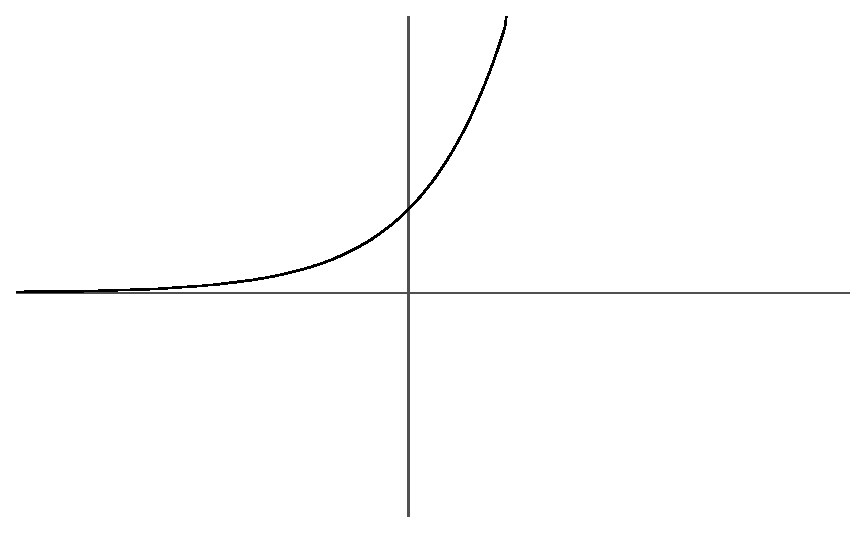
\includegraphics[height=120pt]{SVC.01.03.052.eps}\end{center}
% 
% (a)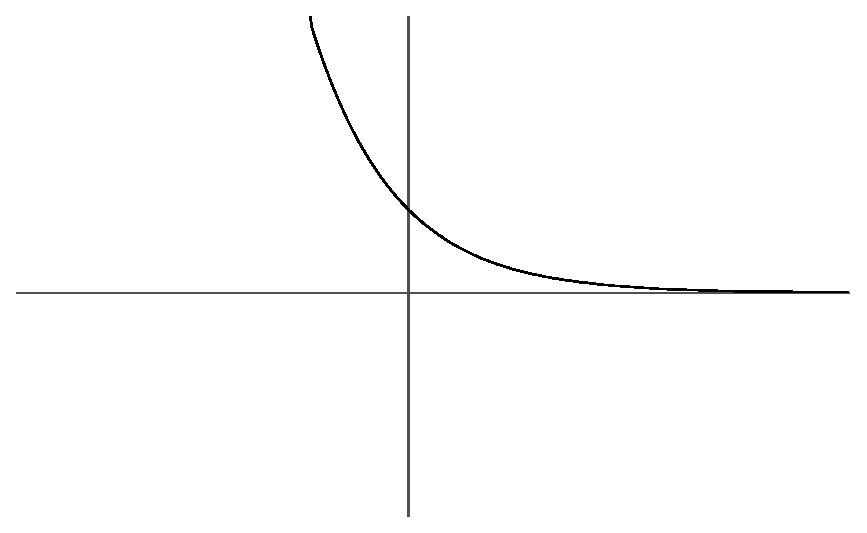
\includegraphics[height=90pt]{SVC.01.03.052a.eps}(b)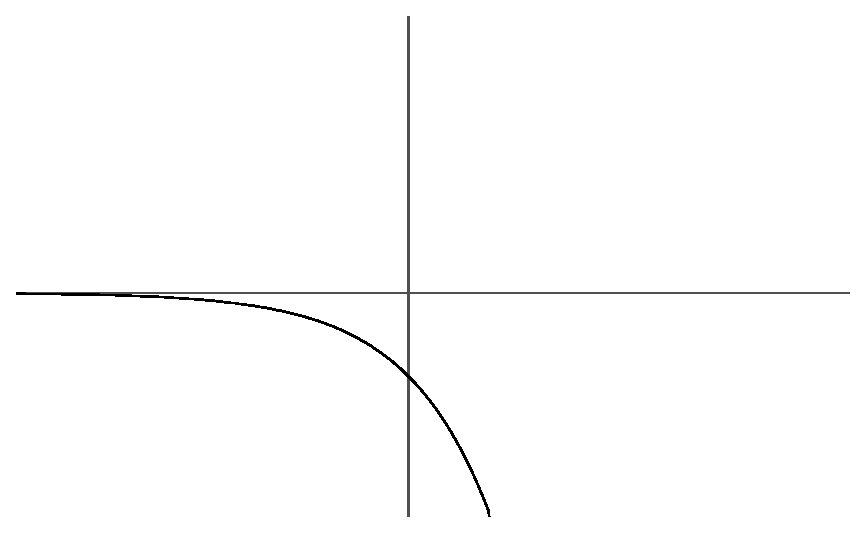
\includegraphics[height=90pt]{SVC.01.03.052b.eps}\\
% (c)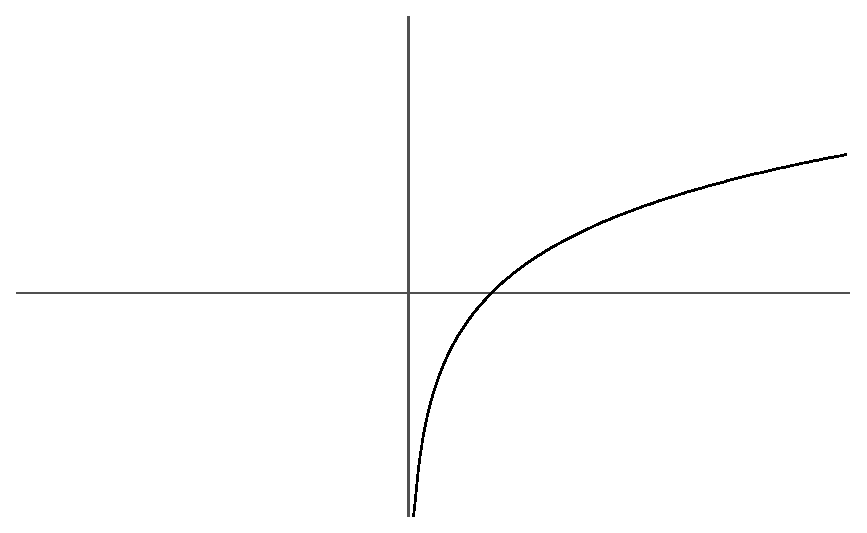
\includegraphics[height=90pt]{SVC.01.03.052c.eps}(d)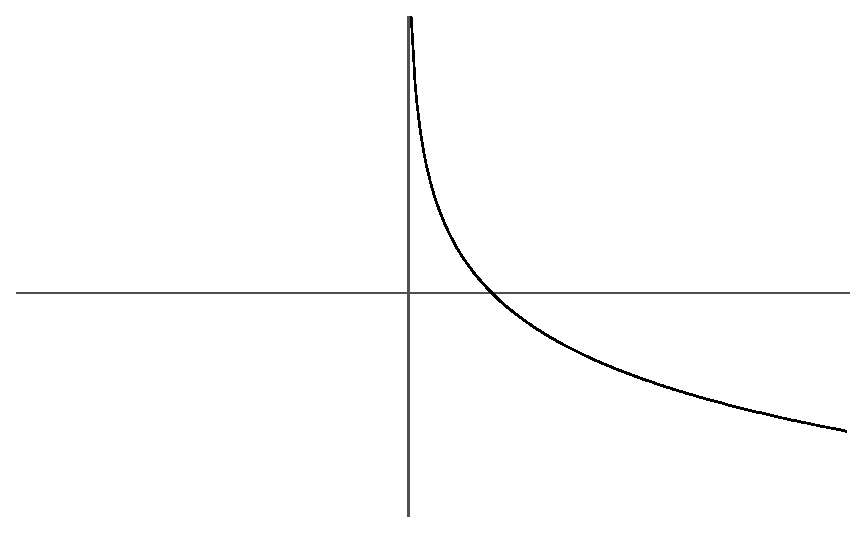
\includegraphics[height=90pt]{SVC.01.03.052d.eps}

%by Project MathVote
